\documentclass[aspectratio=169]{beamer}
\usetheme{TUDelft}

% ====================================================================
% ANIMATION TOGGLE
% ====================================================================
\newif\ifanimated
\animatedtrue
\ifdefined\staticmode
  \animatedfalse
\fi
\newcommand{\cpause}{\ifanimated\pause\fi}

% Packages
\usepackage{amsmath}
\usepackage{amssymb}
\usepackage{algorithm}
\usepackage{algorithmic}
\usepackage{graphicx}
\usepackage{tikz}
\usepackage{booktabs}
\usepackage{listings}
\usepackage{xcolor}
\usepackage{fontawesome5}

% Python code styling
\lstset{
    language=Python,
    basicstyle=\ttfamily\footnotesize,
    keywordstyle=\color{blue},
    commentstyle=\color{gray},
    stringstyle=\color{red},
    showstringspaces=false,
    breaklines=true,
    frame=single,
    numbers=left,
    numberstyle=\tiny\color{gray},
    backgroundcolor=\color{gray!10}
}

% TikZ libraries
\usetikzlibrary{shapes,arrows,positioning,calc,patterns,decorations.pathreplacing,shadows}

% Custom colors
\definecolor{sparse}{RGB}{52,152,219}    % Blue
\definecolor{dense}{RGB}{231,76,60}      % Red
\definecolor{hybrid}{RGB}{46,204,113}    % Green

\usepackage{tikz}
\usetikzlibrary{positioning, shapes, arrows, shadows, fit, calc, decorations.pathreplacing}

% Semantic Colors - One meaning per color
\definecolor{irSparse}{HTML}{3498DB}   % Sparse/BM25: Blue
\definecolor{irDense}{HTML}{E67E22}    % Dense/Embeddings: Orange
\definecolor{irRerank}{HTML}{C0392B}   % Rerank/Cross-encoder: Red
\definecolor{irHybrid}{HTML}{2ECC71}   % Hybrid/Fusion: Green
\definecolor{irANN}{HTML}{9B59B6}      % ANN/Infra: Purple
\definecolor{irInfra}{HTML}{58595B}    % General Infra: Dark Gray
\definecolor{irMuted}{HTML}{D9D9D9}    % Faint Gray

% Base Styles - Consistent Diagram Grammar
\tikzset{
    irBoxBase/.style={
        rectangle, 
        draw, 
        rounded corners=2pt, 
        minimum height=0.8cm, 
        minimum width=2cm,
        font=\small\sffamily,
        align=center,
        drop shadow={opacity=0.15},
        inner sep=5pt
    },
    irDatabase/.style={
        cylinder, 
        draw, 
        shape border rotate=90, 
        aspect=0.25, 
        minimum height=1.2cm, 
        minimum width=1cm,
        fill=irMuted!20,
        draw=irInfra,
        font=\tiny\sffamily,
        align=center
    },
    % Semantic Variants
    sparse/.style={irBoxBase, fill=irSparse!10, draw=irSparse},
    dense/.style={irBoxBase, fill=irDense!10, draw=irDense},
    rerank/.style={irBoxBase, fill=irRerank!10, draw=irRerank},
    hybrid/.style={irBoxBase, fill=irHybrid!10, draw=irHybrid},
    ann/.style={irBoxBase, fill=irANN!10, draw=irANN},
    infra/.style={irBoxBase, fill=irInfra!10, draw=irInfra},
    % Legacy support / Utility
    muted/.style={irBoxBase, fill=irMuted!20, draw=irMuted!80!black, text=irMuted!50!black},
    ghost/.style={irBoxBase, fill=white, draw=irMuted!50, text=irMuted, dashed, drop shadow={opacity=0}},
    emph/.style={draw=irRerank, thick, drop shadow={shadow xshift=0mm, shadow yshift=0mm, fill=irRerank, opacity=0.3}},
    % Arrows
    irArrowBase/.style={->, thick, >=latex, draw=irInfra},
    irLabel/.style={
        font=\tiny\itshape, 
        text=irInfra, 
        align=center, 
        text width=2.5cm, 
        inner sep=3pt
    }
}


% =========================================================
% Stage Badge System
% =========================================================
% \irStage{StageName}
\newcommand{\irStage}[1]{%
    \begin{tikzpicture}[remember picture, overlay]
        \node[
            anchor=north east,
            fill=irInfra!10,
            text=irInfra,
            font=\tiny\bfseries,
            inner sep=3pt,
            rounded corners=1pt,
            yshift=-0.5cm,
            xshift=-0.5cm
        ] at (current page.north east) {#1};
    \end{tikzpicture}%
}

% =========================================================
% Math Highlighting
% =========================================================
% \mathhl[color]{content}
\newcommand{\mathhl}[2][irDense!30]{%
    \colorbox{#1}{$\displaystyle #2$}%
}

% =========================================================
% Math Vectors
% =========================================================
\newcommand{\vs}{\mathbf{s}}

% =========================================================
% Core Box Primitives
% =========================================================
% \IRBox[width]{id}{at}{title}{subtitle}{variant}
% Default width chosen for lecture slides; override when needed.
% \IRBox[width]{id}{at}{title}{subtitle}{variant}[extra options]
\DeclareDocumentCommand{\IRBox}{O{3.5cm} m m m m m O{}}{%
    \node[#6, text width=#1, #7] (#2) at #3 {%
        \textbf{#4}%
        \if\relax\detokenize{#5}\relax
        \else\\[-1mm]\scriptsize #5%
        \fi
    };%
}

% \IRWideBox{id}{at}{width}{title}{subtitle}{variant}
\newcommand{\IRWideBox}[6]{%
    \node[#6, text width=#3] (#1) at #2 {%
        \textbf{#4}%
        \if\relax\detokenize{#5}\relax
        \else\\[-1mm]\scriptsize #5%
        \fi
    };%
}

% =========================================================
% Arrow Primitives
% =========================================================
% Safe default: left-to-right flow
% \IRArrow{from}{to}{label}
\newcommand{\IRArrow}[3]{%
    \draw[irArrowBase] (#1.east) -- node[irArrowLabelAbove] {#3} (#2.west);%
}

% Explicit left-to-right
% \IRArrowLR{from}{to}{label}
\newcommand{\IRArrowLR}[3]{%
    \draw[irArrowBase] (#1.east) -- node[irArrowLabelAbove] {#3} (#2.west);%
}

% Explicit top-to-bottom
% \IRArrowTB{from}{to}{label}
\newcommand{\IRArrowTB}[3]{%
    \draw[irArrowBase] (#1.south) -- node[irArrowLabelRight] {#3} (#2.north);%
}

% Fully explicit anchor-to-anchor path
% \IRArrowPath{from anchor}{to anchor}{label}
% Example: \IRArrowPath{a.east}{b.north}{score}
\newcommand{\IRArrowPath}[3]{%
    \draw[irArrowBase] (#1) -- node[irArrowLabelAbove] {#3} (#2);%
}

% Orthogonal elbow path
% \IRArrowElbow{from anchor}{to anchor}{label}
% Example: \IRArrowElbow{a.east}{b.north}{feedback}
\newcommand{\IRArrowElbow}[3]{%
    \draw[irArrowBase] (#1) -| node[irArrowLabelBox] {#3} (#2);%
}

% Slanted arrow for special cases only
% \IRArrowSlanted{from anchor}{to anchor}{label}{pos}{width}
\newcommand{\IRArrowSlanted}[5]{%
    \draw[irArrowBase] (#1) -- node[above, sloped, irLabel, pos=#4, text width=#5, fill=white, inner sep=1pt] {#3} (#2);%
}

% =========================================================
% Accent Elements
% =========================================================
% \IRBadge{at}{text}
\newcommand{\IRBadge}[2]{%
    \node[
        draw=irAccent,
        fill=irAccent!20,
        rounded corners=1pt,
        font=\tiny\bfseries,
        inner sep=2pt
    ] at #1 {#2};%
}

% =========================================================
% Grouping
% =========================================================
% \IRGroup{fit nodes}{label}{variant}
% Example: \IRGroup{(a)(b)(c)}{First-stage retrieval}{muted}
\newcommand{\IRGroup}[3]{%
    \node[
        irGroupBase,
        #3,
        fit=#1
    ] (group) {};
    \node[
        anchor=north west,
        font=\tiny\bfseries,
        #3
    ] at ([xshift=2pt,yshift=-2pt] group.north west) {#2};%
}

% =========================================================
% Domain-Specific Shapes
% =========================================================
% \IRDocStack{id}{at}{label}
\newcommand{\IRDocStack}[3]{%
    \node[irDocStack] (#1) at #2 {#3};%
}

% \IRDatabase{id}{at}{label}
\newcommand{\IRDatabase}[3]{%
    \node[irDatabase] (#1) at #2 {#3};%
}

% =========================================================
% Layout Helpers
% =========================================================
% \IRPipelineTier{id}{at}{text}{label}{variant}
\newcommand{\IRPipelineTier}[5]{%
    \IRBox{#1}{#2}{#3}{}{#5}[]
    \node[anchor=west, irLabel, xshift=0.5cm] at (#1.east) {#4};%
}

% \IRTelescopeTier{id}{at}{width}{text}{variant}
\newcommand{\IRTelescopeTier}[5]{%
    \node[
        irTelescopeBase,
        #5,
        minimum width=#3
    ] (#1) at #2 {#4};%
}

% \IRStep{id}{at}{title}{subtitle}{variant}
% Creates a numbered step badge left of a box.
\newcommand{\IRStep}[5]{%
    \node[
        circle,
        draw=irAccent,
        fill=irAccent!20,
        font=\tiny\bfseries,
        inner sep=2pt
    ] (#1_num) at #2 {#1};
    \node[
        #5,
        text width=3.5cm,
        right=1.5cm of #1_num
    ] (#1) {%
        \textbf{#3}%
        \if\relax\detokenize{#4}\relax
        \else\\[-1mm]\scriptsize #4%
        \fi
    };
    \draw[irArrowBase, thin] (#1_num.east) -- (#1.west);%
}


% Title information
\title[Indexing]{Information Retrieval Indexing}
\subtitle{Lecture 2: Sparse and Dense Indexing}
\author{Avishek Anand}
\institute{Information Retrieval}
\date{\today}

\begin{document}

% Title slide
\begin{frame}
\titlepage
\end{frame}

% \begin{frame}{The Modern IR Landscape}
% \begin{center}
% 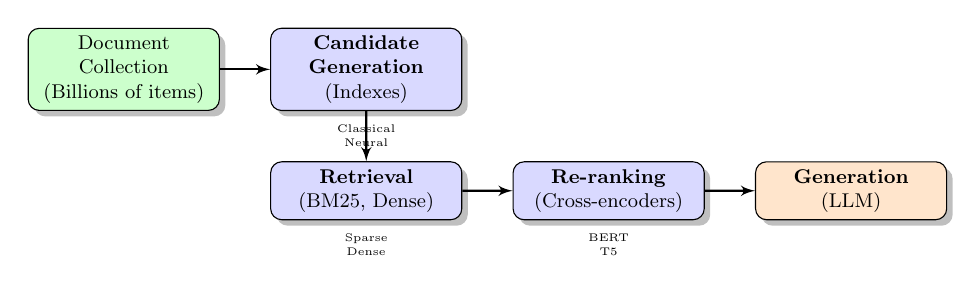
\begin{tikzpicture}[
    scale=0.8, transform shape,
    node distance=0.8cm,
    box/.style={rectangle, draw, rounded corners, fill=blue!15, text width=2.8cm, align=center, minimum height=0.8cm, font=\small, drop shadow},
    arrow/.style={->, thick, >=latex'}
]
    \node[box, fill=green!20] (collection) {Document Collection \\ (Billions of items)};
    \node[box, right=of collection] (gen) {\textbf{Candidate Generation} \\ (Indexes)};
    \node[box, below=of gen] (ret) {\textbf{Retrieval} \\ (BM25, Dense)};
    \node[box, right=of ret] (rank) {\textbf{Re-ranking} \\ (Cross-encoders)};
    \node[box, right=of rank, fill=orange!20] (llm) {\textbf{Generation} \\ (LLM)};
    
    \draw[arrow] (collection) -- (gen);
    \draw[arrow] (gen) -- (ret);
    \draw[arrow] (ret) -- (rank);
    \draw[arrow] (rank) -- (llm);
    
    \node[below=0.1cm of gen, font=\tiny, text width=2.6cm, align=center] {Classical \\ Neural};
    \node[below=0.1cm of ret, font=\tiny, text width=2.6cm, align=center] {Sparse \\ Dense};
    \node[below=0.1cm of rank, font=\tiny, text width=2.6cm, align=center] {BERT \\ T5};
\end{tikzpicture}

% \end{center}

% \vspace{1em}

% \textbf{Our Focus Today:} The engine room of this pipeline --- \textbf{Candidate Generation}.
% \end{frame}

\begin{frame}{Retrieval $\rightarrow$ Re-ranking $\rightarrow$ Reasoning}
\begin{center}
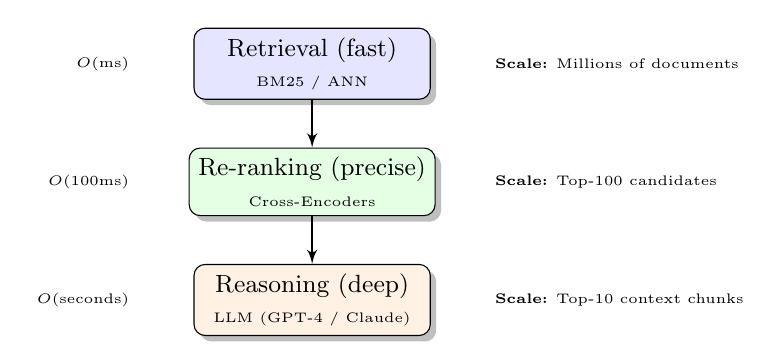
\begin{tikzpicture}[
    node distance=0.8cm,
    label/.style={font=\tiny, gray},
    vstep/.style={rectangle, draw, rounded corners, minimum width=3cm, minimum height=0.8cm, align=center, font=\small, drop shadow}
]
    \node[vstep, fill=blue!10] (ret) at (0, 3) {Retrieval (fast) \\ \tiny BM25 / ANN};
    \node[vstep, fill=green!10] (rank) at (0, 1.5) {Re-ranking (precise) \\ \tiny Cross-Encoders};
    \node[vstep, fill=orange!10] (llm) at (0, 0) {Reasoning (deep) \\ \tiny LLM (GPT-4 / Claude)};
    
    \draw[->, thick, >=latex'] (ret) -- (rank);
    \draw[->, thick, >=latex'] (rank) -- (llm);
    
    \node[anchor=west] at (2.2, 3) {\tiny \textbf{Scale:} Millions of documents};
    \node[anchor=west] at (2.2, 1.5) {\tiny \textbf{Scale:} Top-100 candidates};
    \node[anchor=west] at (2.2, 0) {\tiny \textbf{Scale:} Top-10 context chunks};
    
    \node[anchor=east] at (-2.2, 3) {\tiny $O(\text{ms})$};
    \node[anchor=east] at (-2.2, 1.5) {\tiny $O(100\text{ms})$};
    \node[anchor=east] at (-2.2, 0) {\tiny $O(\text{seconds})$};
\end{tikzpicture}

\end{center}

\vspace{0.5em}
\begin{alertblock}{Key Principle}
\textbf{Indexing sets the ceiling.} Everything else (re-ranking, LLM reasoning) can only refine the results that retrieval finds.
\end{alertblock}
\end{frame}

\begin{frame}{Traditional Retrieval: 10 Blue Links}
\begin{columns}[T,onlytextwidth]
\begin{column}{0.45\textwidth}
\begin{center}
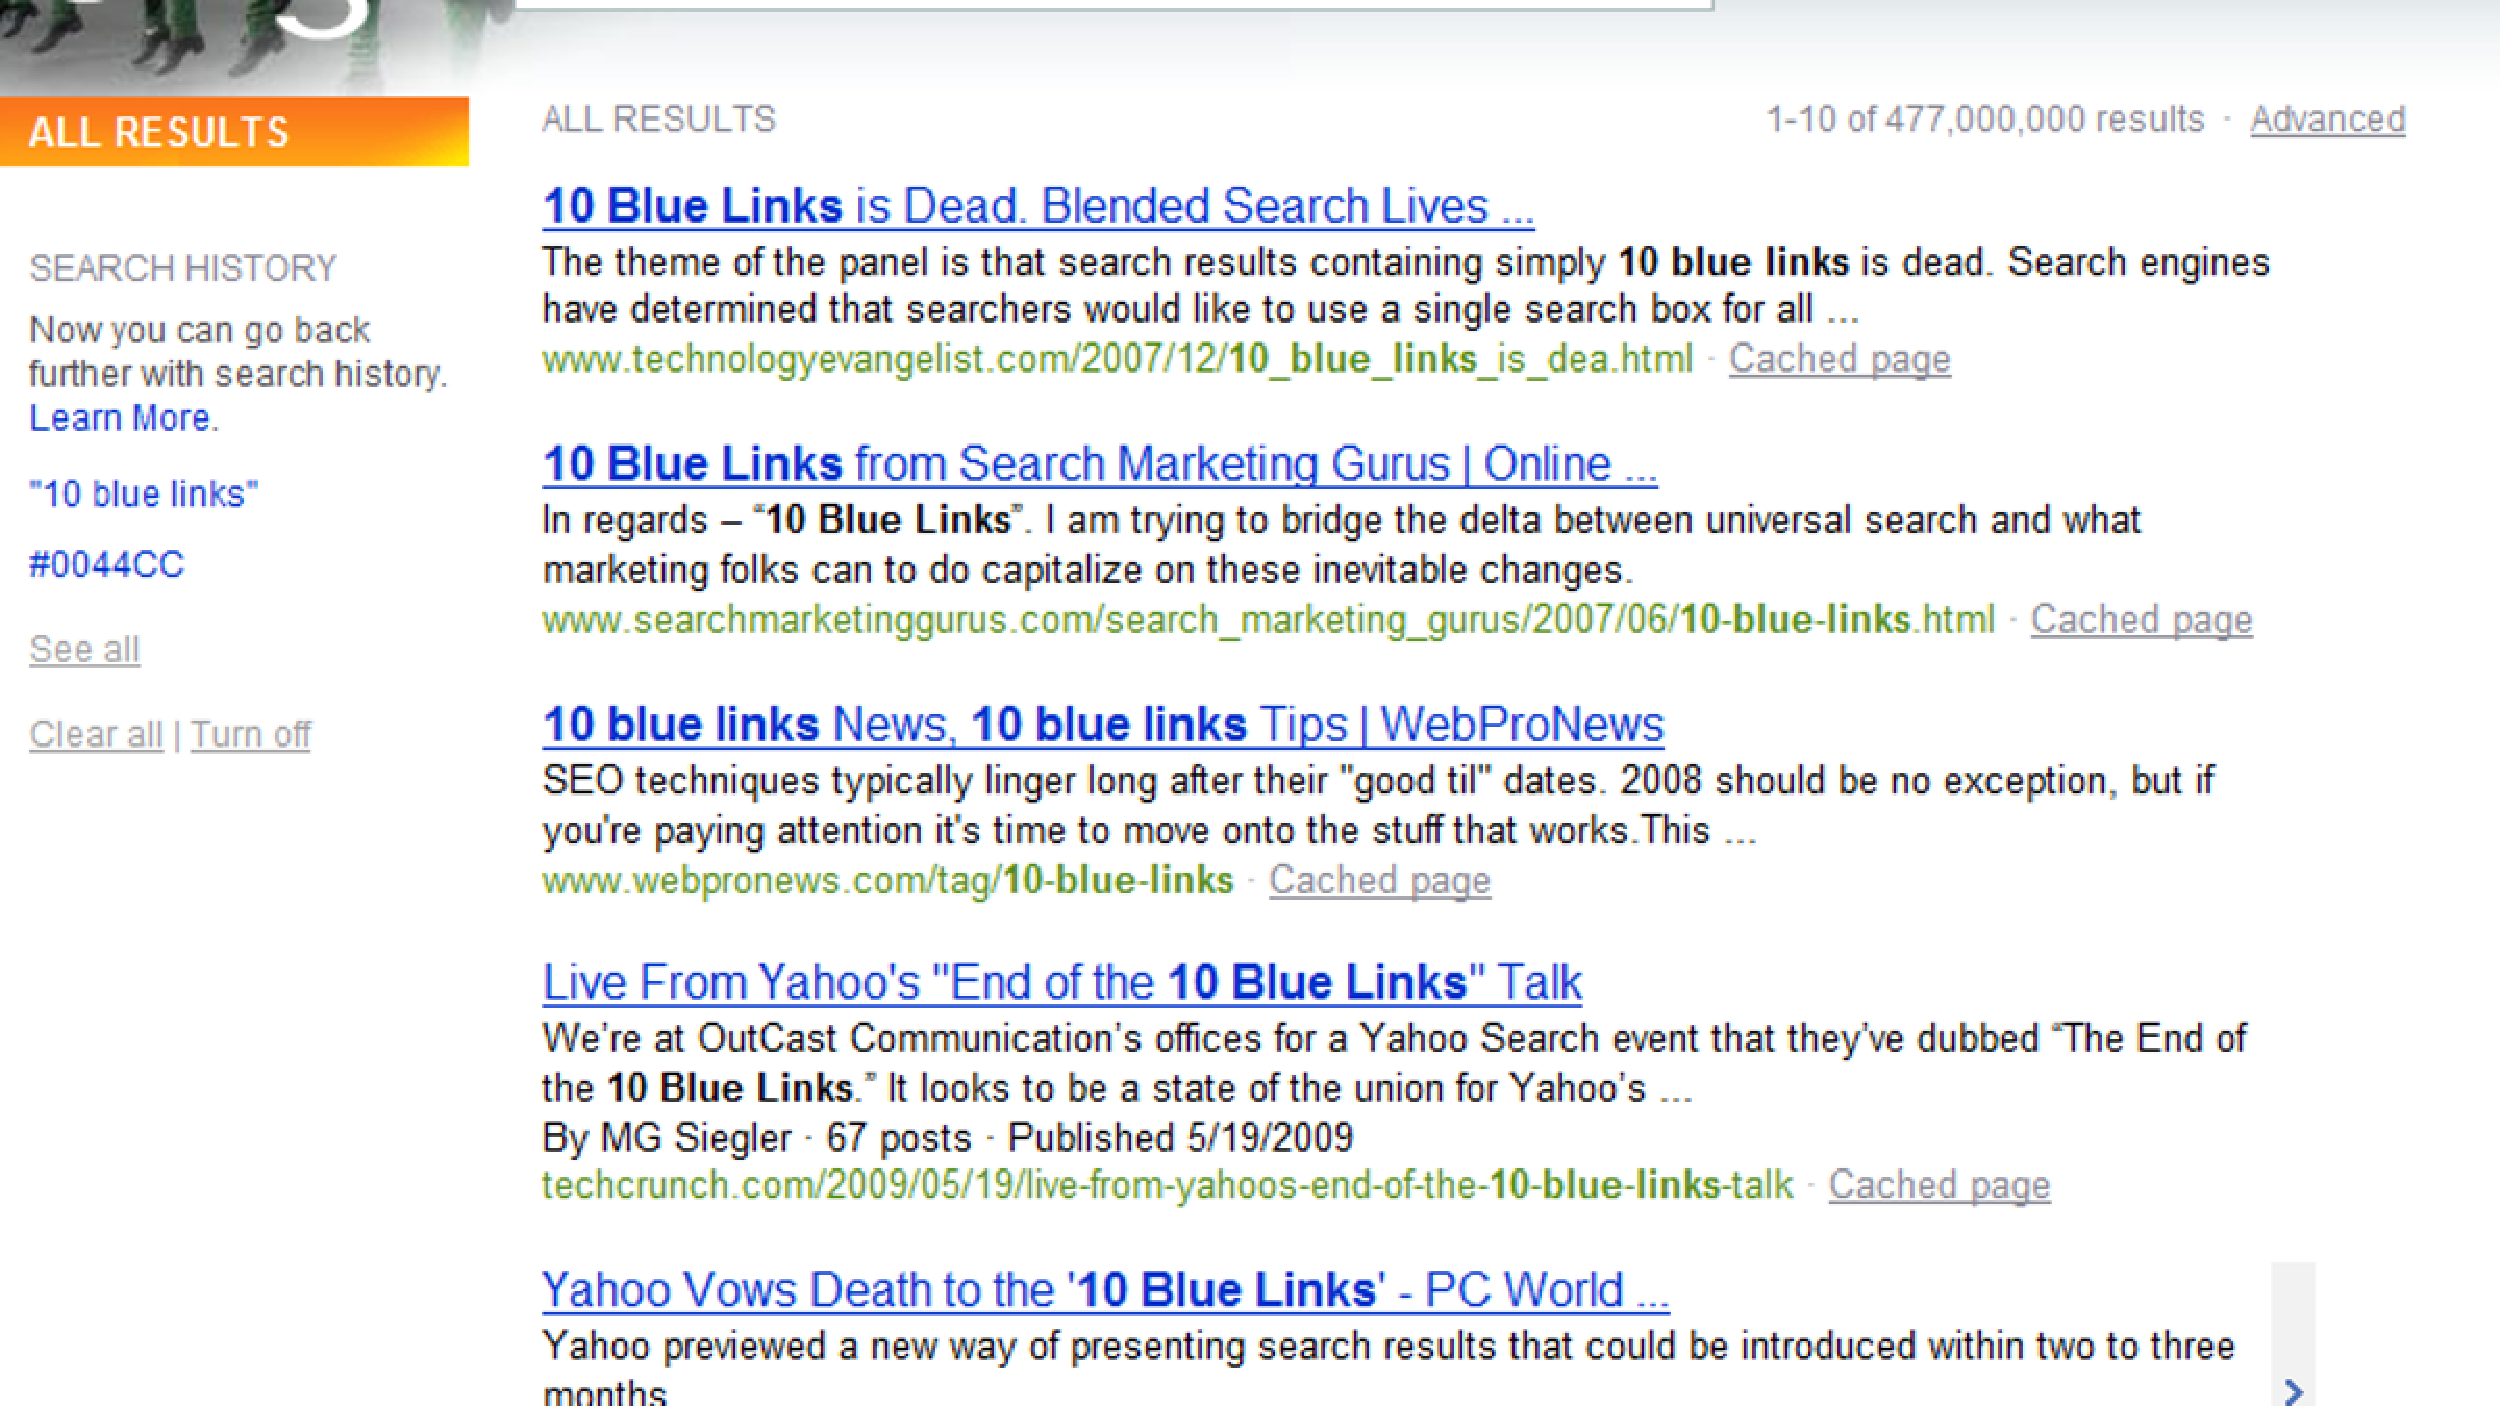
\includegraphics[width=0.9\textwidth]{figures/trad-retrieval.pdf}
\end{center}
\end{column}
\begin{column}{0.5\textwidth}
\begin{itemize}
    \item \textbf{User Task:} Search for information.
    \item \textbf{Output:} A list of relevant documents.
    \item \textbf{Interaction:} User clicks links, reads, and synthesizes.
    \item \textbf{Classic System:} Google, Bing, Yahoo in the 2000s.
\end{itemize}
\end{column}
\end{columns}

\vspace{1em}
\begin{alertblock}{Problem}
User does all the hard work of reading and combining information!
\end{alertblock}
\end{frame}

\begin{frame}{Modern IR: Retrieval-Augmented Generation (RAG)}
\begin{columns}[T,onlytextwidth]
\begin{column}{0.45\textwidth}
\begin{center}
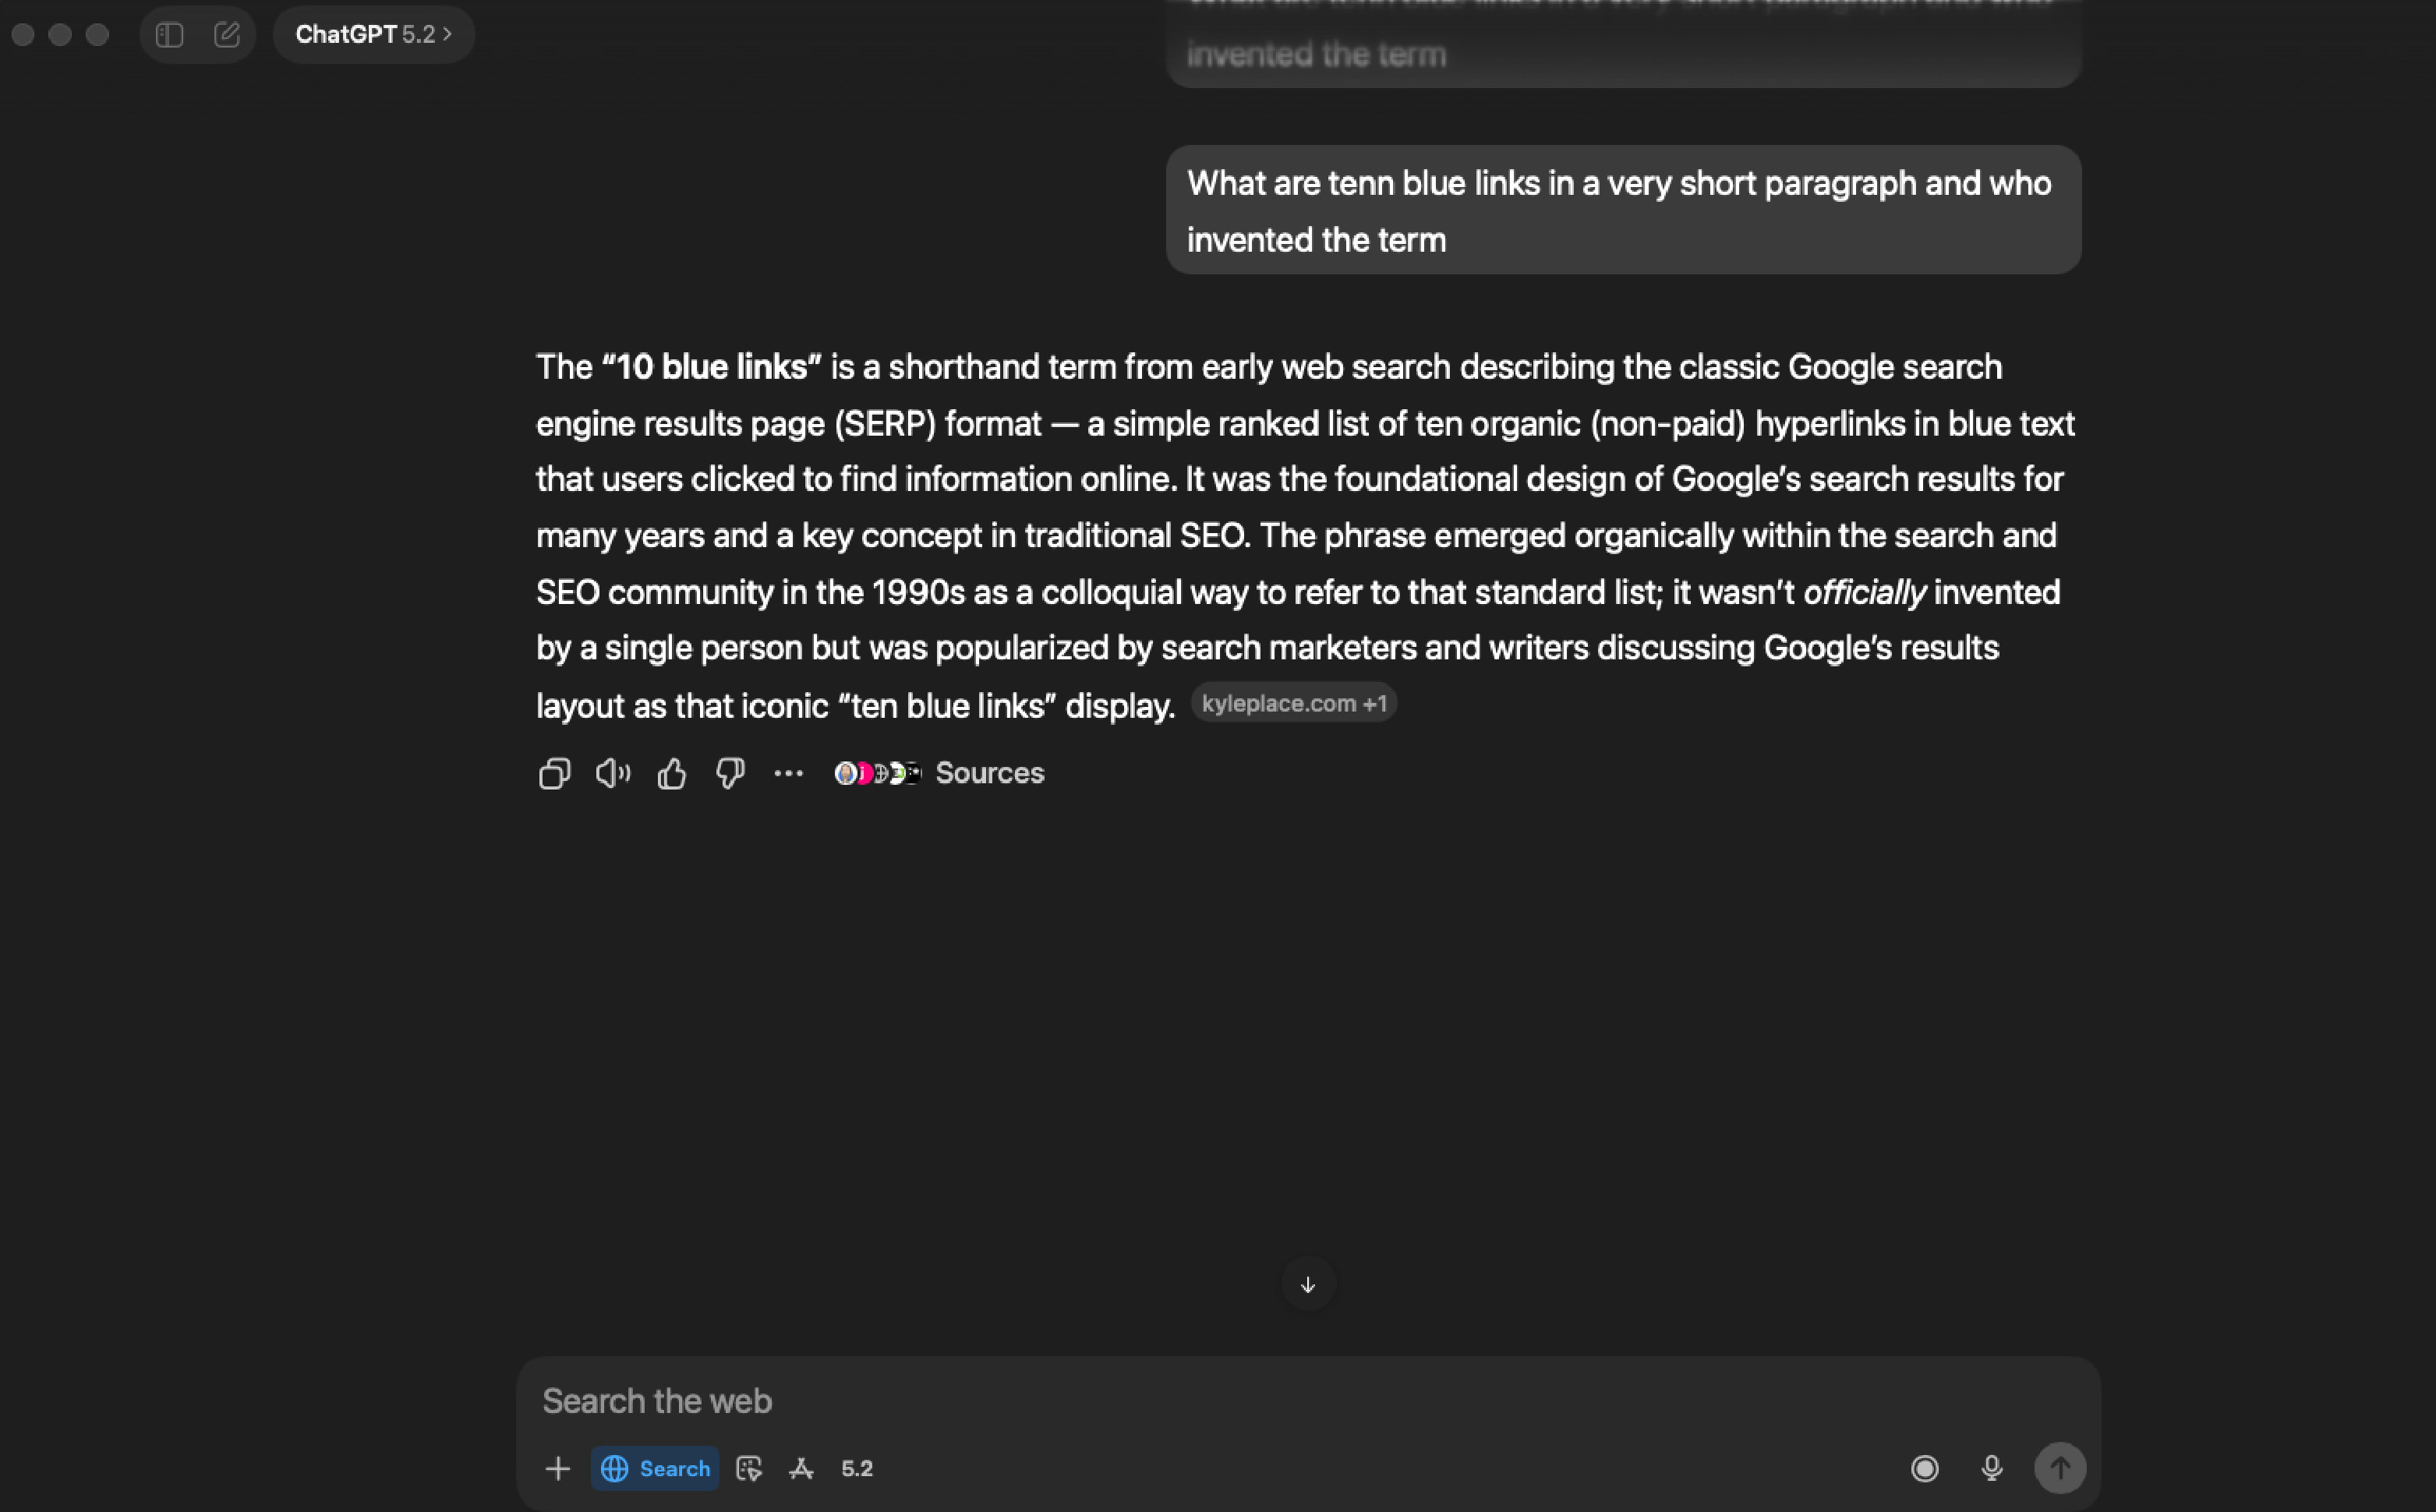
\includegraphics[width=0.9\textwidth]{figures/modern-rag.pdf}
\end{center}
\end{column}
\begin{column}{0.5\textwidth}
\begin{itemize}
    \item \textbf{User Task:} Ask a question.
    \item \textbf{Output:} A synthesized answer in natural language.
    \item \textbf{Process:}
    \begin{enumerate}
        \item \textbf{Retrieve} relevant facts.
        \item \textbf{Augment} LLM prompt with facts.
        \item \textbf{Generate} final answer.
    \end{enumerate}
    \item \textbf{Modern System:} ChatGPT, Perplexity, Bing Chat.
\end{itemize}
\end{column}
\end{columns}
\end{frame}

\begin{frame}{The Interface Changed. The Engine Did Not.}
\begin{columns}[T,onlytextwidth]
\begin{column}{0.48\textwidth}
\textbf{Old Interface (2000s):}
\begin{itemize}
    \item Output: Ranked documents
    \item Interaction: User reads/clicks
\end{itemize}

\begin{center}
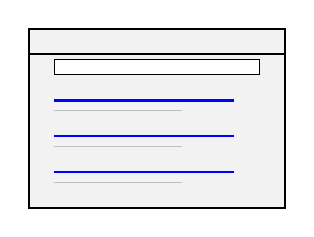
\begin{tikzpicture}[scale=0.65, every node/.style={transform shape}]
    % Mock browser
    \draw[thick, fill=gray!10] (0,0) rectangle (5,3.5);
    \draw[thick] (0,3) -- (5,3);
    \draw[fill=white] (0.5, 2.6) rectangle (4.5, 2.9);
    \foreach \y in {0.5, 1.2, 1.9} {
        \draw[blue, thick] (0.5, \y+0.2) -- (4, \y+0.2);
        \draw[gray!50] (0.5, \y) -- (3, \y);
    }
\end{tikzpicture}

\end{center}
\end{column}

\begin{column}{0.48\textwidth}
\textbf{Modern Interface (2024+):}
\begin{itemize}
    \item Output: Generated answers
    \item Interaction: Model synthesizes facts
\end{itemize}

\begin{center}
\begin{tikzpicture}[scale=0.65, every node/.style={transform shape}]
    % Mock chat
    \draw[thick, fill=gray!10] (0,0) rectangle (5,3.5);
    \draw[thick] (0,3) -- (5,3);
    \draw[fill=blue!10, rounded corners] (0.5, 2.4) rectangle (4.5, 2.9);
    \node at (2.5, 2.65) {\tiny \faUser \textit{ what is IR?}};
    \draw[fill=green!10, rounded corners] (0.5, 0.5) rectangle (4.5, 1.8);
    \node[text width=3.8cm] at (2.5, 1.15) {\tiny \faRobot \textbf{A:} IR is the field of finding relevant information...};
\end{tikzpicture}

\end{center}
\end{column}
\end{columns}

\vspace{1em}
\begin{alertblock}{Core Message}
\textbf{Retrieval now serves models instead of users.} \\
But the underlying components (Index, Retrieval, Relevance) remain the same.
\end{alertblock}
\end{frame}

\begin{frame}{Why Do We Need Indexing?}
\begin{enumerate}
    \item \textbf{Scale:} Cannot score all documents in real-time.
    \item \textbf{Latency:} Users (and LLMs) expect sub-second responses.
    \item \textbf{Feasibility:} Must reduce millions $\rightarrow$ hundreds of candidates.
\end{enumerate}

\vspace{1em}

\begin{center}
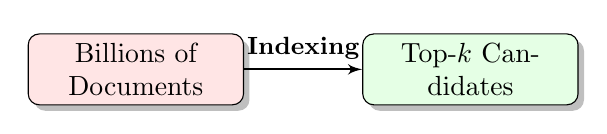
\begin{tikzpicture}[
    node distance=1.5cm,
    box/.style={rectangle, draw, rounded corners, fill=blue!15, text width=2.5cm, align=center, minimum height=0.8cm, drop shadow},
    arrow/.style={->, thick, >=latex'}
]
    \node[box, fill=red!10] (all) {Billions of Documents};
    \node[box, right=of all, fill=green!10] (few) {Top-$k$ Candidates};
    \draw[arrow] (all) -- node[above, font=\small\bf] {Indexing} (few);
\end{tikzpicture}

\end{center}

\vspace{2em}

\begin{exampleblock}{The Bottom Line}
\textbf{Indexing is not just an optimization. It is the bridge to feasibility.}
\end{exampleblock}
\end{frame}

\begin{frame}{What Does Indexing Control?}
\begin{block}{Indexing Determines}
\begin{itemize}
    \item \textbf{Recall Ceiling:} Which documents can ever be retrieved.
    \item \textbf{Latency Budget:} How many candidates can be scored (fast vs slow).
    \item \textbf{Cost per Query:} Hardware requirements and compute cost.
    \item \textbf{What the LLM is allowed to see:} Retrieval is the LLM's "eyes".
\end{itemize}
\end{block}

\vspace{1em}

\begin{center}
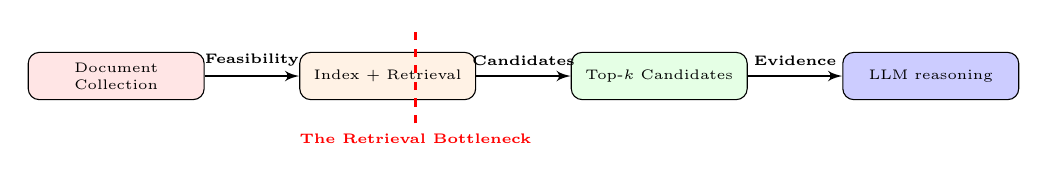
\begin{tikzpicture}[
    node distance=1.2cm,
    box/.style={rectangle, draw, rounded corners, fill=blue!10, text width=2cm, align=center, minimum height=0.6cm, font=\tiny},
    arrow/.style={->, thick, >=latex'}
]
    \node[box, fill=red!10] (coll) {Document Collection};
    \node[box, right=of coll, fill=orange!10] (idx) {Index + Retrieval};
    \node[box, right=of idx, fill=green!10] (top) {Top-$k$ Candidates};
    \node[box, right=of top, fill=blue!20] (llm) {LLM reasoning};
    
    \draw[arrow] (coll) -- node[above, font=\tiny\bf] {Feasibility} (idx);
    \draw[arrow] (idx) -- node[above, font=\tiny\bf] {Candidates} (top);
    \draw[arrow] (top) -- node[above, font=\tiny\bf] {Evidence} (llm);
    
    \draw[dashed, red, thick] (3.8, -0.6) -- (3.8, 0.6) node[below=1.2cm, font=\tiny\bf, text=red] {The Retrieval Bottleneck};
\end{tikzpicture}

\end{center}

\vspace{0.5em}

\begin{alertblock}{Hard Constraint}
If retrieval misses it, the LLM cannot reason about it.
\end{alertblock}
\end{frame}

% \begin{frame}{Course Context (Updated)}
% \begin{enumerate}
%     \item Introduction to IR: Vector Space Model \& Boolean Retrieval \faCheck 
%     \item \textbf{Modern Indexing for RAG} $\leftarrow$ Today
%     \item Ranking: BM25, Query Expansion, Language Models
%     \item Embeddings \& Transformer-based Re-rankers
%     \item Dense Retrieval (Deep Dive)
%     \item Learning to Rank
% \end{enumerate}

% \vspace{1em}

% \textbf{Today's Focus:} Candidate Generation stage (Indexes).
% \end{frame}

\begin{frame}{Outline}
\tableofcontents
\end{frame}

% ====================================================================
% SECTION 1: SPARSE INDEXING (CLASSICAL)
% ====================================================================
\section{Sparse Indexing: The Classical Approach}

\begin{frame}{The Inverted Index: Still Relevant in 2024}
\begin{block}{What Powers These Systems?}
\begin{itemize}
    \item Google Search
    \item Elasticsearch / OpenSearch
    \item Database full-text search (PostgreSQL, MySQL)
    \item RAG sparse retrieval component
\end{itemize}
Answer: \textbf{Inverted indexes}
\end{block}

\vspace{1em}

\textbf{Why still relevant in the age of neural networks?}
\begin{enumerate}
    \item \textcolor{green}{\textbf{Exact matching:}} Find "iPhone 15 Pro Max" precisely
    \item \textcolor{green}{\textbf{Speed:}} 5-10ms queries on millions of documents
    \item \textcolor{green}{\textbf{Explainability:}} Can see which terms matched
    \item \textcolor{green}{\textbf{Hybrid search:}} Complements dense retrieval
\end{enumerate}
\end{frame}

\begin{frame}[shrink=15]{Inverted Index: Core Structure}
\textbf{Documents:}
\begin{itemize}
    \item Doc1: ``neural networks for deep learning''
    \item Doc2: ``deep learning applications''
    \item Doc3: ``neural machine translation''
\end{itemize}

\vspace{1em}

\begin{center}
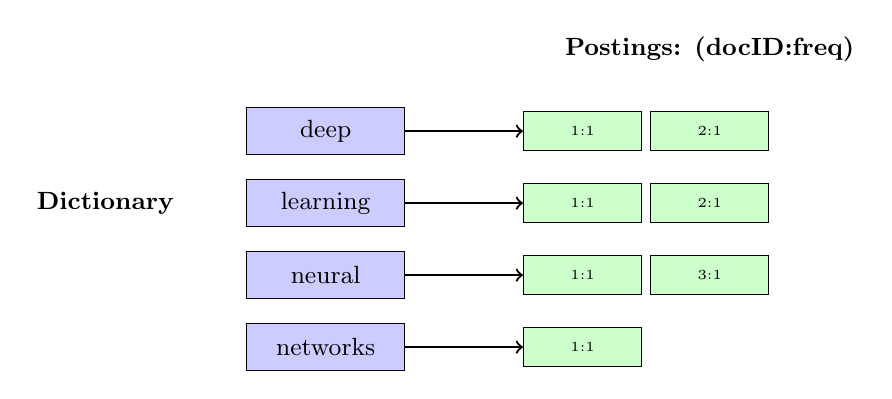
\begin{tikzpicture}[
    node distance=0.3cm,
    dict/.style={rectangle, draw, fill=blue!20, minimum width=2cm, minimum height=0.6cm, font=\small},
    post/.style={rectangle, draw, fill=green!20, minimum width=1.5cm, minimum height=0.5cm, font=\tiny}
]
    % Dictionary
    \node[dict] (t1) {deep};
    \node[dict, below=of t1] (t2) {learning};
    \node[dict, below=of t2] (t3) {neural};
    \node[dict, below=of t3] (t4) {networks};
    
    \node[left=0.8cm of t2.west, font=\small\bf] {Dictionary};
    
    % Postings
    \node[post, right=1.5cm of t1] (p11) {1:1};
    \node[post, right=0.1cm of p11] (p12) {2:1};
    
    \node[post, right=1.5cm of t2] (p21) {1:1};
    \node[post, right=0.1cm of p21] (p22) {2:1};
    
    \node[post, right=1.5cm of t3] (p31) {1:1};
    \node[post, right=0.1cm of p31] (p32) {3:1};
    
    \node[post, right=1.5cm of t4] (p41) {1:1};
    
    \node[above=0.5cm of p12, font=\small\bf] {Postings: (docID:freq)};
    
    % Arrows
    \draw[->, thick] (t1) -- (p11);
    \draw[->, thick] (t2) -- (p21);
    \draw[->, thick] (t3) -- (p31);
    \draw[->, thick] (t4) -- (p41);
\end{tikzpicture}

\end{center}

\vspace{1em}

\textbf{Query:} ``neural learning'' \\
\textbf{Process:} Lookup ``neural'' $\rightarrow$ [1, 3], lookup ``learning'' $\rightarrow$ [1, 2] \\
\textbf{Intersection:} [1] $\leftarrow$ Doc 1 contains both terms
\end{frame}

\begin{frame}[shrink=10]{Inverted Index as a Sparse Matrix}
\begin{block}{Vector Space Interpretation}
\begin{itemize}
    \item Documents = Rows ($D$)
    \item Terms = Columns ($V$)
    \item Values = Weights (TF-IDF, BM25)
\end{itemize}
\end{block}

\begin{center}
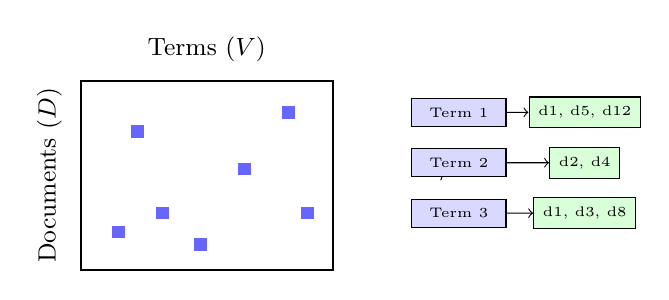
\begin{tikzpicture}[scale=0.8]
    % Matrix outline
    \draw[thick] (0,0) rectangle (4,3);
    \node[rotate=90] at (-0.5, 1.5) {\small Documents ($D$)};
    \node at (2, 3.5) {\small Terms ($V$)};
    
    % Sparse points
    \foreach \x/\y in {0.5/0.5, 1.2/0.8, 0.8/2.1, 2.5/1.5, 3.2/2.4, 1.8/0.3, 3.5/0.8} {
        \fill[blue!60] (\x, \y) rectangle (\x+0.2, \y+0.2);
    }
    
    \node[right=4.2cm] at (0, 1.5) {$\rightarrow$};
    
    % Index structure
    \begin{scope}[shift={(6,0.5)}]
        \node[draw, fill=blue!15, minimum width=1.2cm] (t1) at (0, 2) {\tiny Term 1};
        \node[draw, fill=blue!15, minimum width=1.2cm] (t2) at (0, 1.2) {\tiny Term 2};
        \node[draw, fill=blue!15, minimum width=1.2cm] (t3) at (0, 0.4) {\tiny Term 3};
        
        \node[draw, fill=green!15] (p1) at (2, 2) {\tiny d1, d5, d12};
        \node[draw, fill=green!15] (p2) at (2, 1.2) {\tiny d2, d4};
        \node[draw, fill=green!15] (p3) at (2, 0.4) {\tiny d1, d3, d8};
        
        \draw[->] (t1) -- (p1);
        \draw[->] (t2) -- (p2);
        \draw[->] (t3) -- (p3);
    \end{scope}
\end{tikzpicture}

\end{center}

\begin{exampleblock}{Key Insight}
The Inverted Index is a \textbf{Compressed Sparse Column (CSC)} storage of the Document-Term matrix. We avoid storing zeros!
\end{exampleblock}
\end{frame}

\begin{frame}[shrink=10]{Why Inverted Index is Fast}
\begin{columns}
\begin{column}{0.48\textwidth}
\textbf{Naive Approach:}
\begin{enumerate}
    \item Scan all documents
    \item Check if query terms present
    \item Rank matches
\end{enumerate}
\cpause

\vspace{0.5em}

\textbf{Complexity:} $O(N \cdot M)$
\begin{itemize}
    \item $N$ = number of documents
    \item $M$ = avg document length
\end{itemize}

\vspace{0.5em}

For 10M docs, 500 words each: \\
5 \textbf{billion} comparisons!
\end{column}

\begin{column}{0.48\textwidth}
\textbf{Inverted Index:}
\begin{enumerate}
    \item Lookup term in dictionary
    \item Fetch posting list
    \item Merge posting lists
\end{enumerate}

\vspace{0.5em}

\textbf{Complexity:} $O(k \cdot p)$
\begin{itemize}
    \item $k$ = query terms (typically 2-5)
    \item $p$ = avg posting list size
\end{itemize}

\vspace{0.5em}

For query ``neural learning'': \\
Lookup 2 terms, merge ~1000 docs \\
$\rightarrow$ \textbf{1000$\times$ faster!}
\end{column}
\end{columns}
\end{frame}

\begin{frame}[shrink=10]{Posting List Formats: Evolution}
\begin{block}{Level 1: DocID Only (Boolean Retrieval)}
\texttt{neural: [1, 3, 5, 12, 27, 89]}
\begin{itemize}
    \item Supports: AND, OR, NOT queries
    \item Cannot: Rank by relevance
\end{itemize}
\end{block}

\begin{block}{Level 2: With Frequencies (Ranked Retrieval)}
\texttt{neural: [(1, tf=2), (3, tf=1), (5, tf=3), (12, tf=1), ...]}
\begin{itemize}
    \item Supports: TF-IDF, BM25 scoring
    \item \textbf{This is what we use in practice}
\end{itemize}
\end{block}

\begin{block}{Level 3: With Positions (Phrase Queries)}
\texttt{neural: [(1, tf=2, pos=[5,42]), (3, tf=1, pos=[8]), ...]}
\begin{itemize}
    \item Supports: ``neural networks'' (exact phrase)
    \item Enables: Proximity scoring
    \item Cost: 2-3$\times$ larger index
\end{itemize}
\end{block}
\end{frame}

\begin{frame}{Score Aggregation: Connecting Indexing and VSM}
\begin{block}{Vector Space Model Scoring}
\[ \text{score}(q, d) = \sum_{t \in q \cap d} \text{weight}(t, q) \times \text{weight}(t, d) \]
\end{block}

\begin{columns}[T]
\begin{column}{0.48\textwidth}
\textbf{How it works in the engine:}
\begin{enumerate}
    \item Initialize \textbf{Accumulators} (Doc $\rightarrow$ Score)
    \item For each term $t$ in query:
    \item Traverse postings of $t$
    \item Add contribution to Doc score
\end{enumerate}
\end{column}
\begin{column}{0.48\textwidth}
\textbf{Example:}

\textbf{Query:} ``neural learning''

\vspace{0.3em}

\textbf{Accumulators:}
\begin{itemize}
    \item[] Doc1: 0.0
    \item[] Doc2: 0.0
    \item[] Doc3: 0.0
\end{itemize}

\vspace{0.3em}

\textbf{Process ``neural'':}
\begin{itemize}
    \item[] Doc1: +2.5
    \item[] Doc3: +2.5
\end{itemize}

\vspace{0.3em}

\textbf{Process ``learning'':}
\begin{itemize}
    \item[] Doc1: +3.0
    \item[] Doc2: +3.0
\end{itemize}

\vspace{0.3em}

\textbf{Final:} Doc1=5.5, Doc2=3.0, Doc3=2.5
\end{column}
\end{columns}

\vspace{0.5em}
\begin{exampleblock}{The Power of Sparse Indexing}
We only compute scores for documents that contain at least one query term!
\end{exampleblock}
\end{frame}

\begin{frame}[shrink=20]{Text Preprocessing Pipeline}

\textbf{Raw text:} ``The Neural Networks are Learning!''

\vspace{1em}

\begin{columns}[T,onlytextwidth]
\begin{column}{0.55\textwidth}

\begin{tikzpicture}[scale=0.6, transform shape, spacing/.style={yshift=-2.5cm}]
    % Sequential Boxes using API
    \IRBox{raw}{(0,0)}{The Neural Networks \\ are Learning!}{String Input}{accent}
    
    \begin{scope}[spacing]
        \IRBox{token}{($ (raw) + (0,-2.5) $)}{[The, Neural, Networks, \\ are, Learning, !]}{Tokenized}{primary}
        \IRBox{lower}{($ (token) + (0,-2.5) $)}{[the, neural, networks, \\ are, learning, !]}{Normalized}{primary}
        \IRBox{stop}{($ (lower) + (0,-2.5) $)}{[neural, networks, \\ learning]}{Filtered}{primary}
        \IRBox{stem}{($ (stop) + (0,-2.5) $)}{[neural, network, \\ learn]}{Stemmed}{emph}
    \end{scope}

    % Connect with sloped labels using TB arrows for vertical flow
    \IRArrowTB{raw}{token}{Tokenize}
    \IRArrowTB{token}{lower}{Lowercase}
    \IRArrowTB{lower}{stop}{Stopwords}
    \IRArrowTB{stop}{stem}{Stem/Lemmatize}
\end{tikzpicture}


\end{column}
\hfill
\begin{column}{0.43\textwidth}

\textbf{Pipeline steps:}
\begin{itemize}
    \item \textbf{Tokenization:} Split text into words or symbols.
    \item \textbf{Lowercasing:} Normalize capitalization.
    \item \textbf{Stop word removal:} Eliminate common, low-information words.
    \item \textbf{Stemming/Lemmatization:} Reduce words to their root form.
\end{itemize}

\vspace{0.5em}
\textbf{Critical:} Apply the same preprocessing to query and document text for consistency!

\end{column}
\end{columns}

\end{frame}


\begin{frame}[shrink=25]{Text Preprocessing: Key Decisions}
\begin{block}{1. Tokenization}
\textbf{Simple:} Split on whitespace \\
\textbf{Reality:} Language-dependent
\begin{itemize}
    \item English: ``don't'' $\rightarrow$ ``do'' + ``n't'' or ``dont''?
    \item German: ``Informationssystem'' $\rightarrow$ split compound?
    \item Chinese/Japanese: No spaces between words!
\end{itemize}
\end{block}

\begin{block}{2. Stemming vs. Lemmatization}
\begin{columns}
\begin{column}{0.48\textwidth}
\textbf{Stemming (Porter):}
\begin{itemize}
    \item running $\rightarrow$ run
    \item \textcolor{red}{university $\rightarrow$ univers}
    \item Fast, crude
\end{itemize}
\end{column}
\begin{column}{0.48\textwidth}
\textbf{Lemmatization:}
\begin{itemize}
    \item running $\rightarrow$ run
    \item better $\rightarrow$ good
    \item Accurate, slower
\end{itemize}
\end{column}
\end{columns}
\end{block}

\begin{alertblock}{For Neural Models (BERT, embeddings)}
\textbf{Do NOT stem!} Pre-trained models expect natural text
\end{alertblock}
\end{frame}

\begin{frame}[shrink=10]{Stop Words: Modern Perspective}
\begin{columns}
\begin{column}{0.48\textwidth}
\textbf{Traditional View (pre-2010):}
\begin{itemize}
    \item Remove common words: \\
    the, a, an, is, are, of, in, ...
    \item \textcolor{green}{\faCheck } Smaller index
    \item \textcolor{green}{\faCheck } Less noise
\end{itemize}

\vspace{1em}

\textbf{Problem:}
\begin{itemize}
    \item ``to be or not to be'' $\rightarrow$ ``''
    \item ``The Who'' (band) $\rightarrow$ ``Who''
    \item Loses phrase meaning
\end{itemize}
\end{column}

\begin{column}{0.48\textwidth}
\textbf{Modern View (2010+):}
\begin{itemize}
    \item \textbf{Keep stop words}
    \item Storage is cheap
    \item Important for phrases
    \item Neural models need them
\end{itemize}

\vspace{1em}

\textbf{When to remove:}
\begin{itemize}
    \item Very large scale (web search)
    \item Memory-constrained devices
    \item Proven unnecessary for domain
\end{itemize}
\end{column}
\end{columns}

\vspace{1em}

\begin{block}{Recommendation}
\textbf{Default: Keep stop words} unless you have a specific reason to remove them
\end{block}
\end{frame}

\begin{frame}[fragile]{Preprocessing Depends on Representation}
\begin{columns}[T]
\begin{column}{0.48\textwidth}
\begin{block}{Sparse Retrieval}
\begin{itemize}
    \item \faCut \textbf{Tokenization:} Defines vocabulary entries.
    \item \faLayerGroup \textbf{Stemming:} Useful for term matching (e.g., learn/learning).
    \item \faTrash[regular] \textbf{Stopwords:} Optional (to save space).
\end{itemize}
\end{block}
\end{column}

\begin{column}{0.48\textwidth}
\begin{block}{Dense Retrieval}
\begin{itemize}
    \item \faRobot \textbf{Tokenizer:} Fixed by the model (BPE, WordPiece).
    \item \faBan \textbf{No Stemming:} Models understand word variants.
    \item \faStream \textbf{Truncation:} Context window limits matter.
\end{itemize}
\end{block}
\end{column}
\end{columns}

\vspace{1em}

\begin{center}
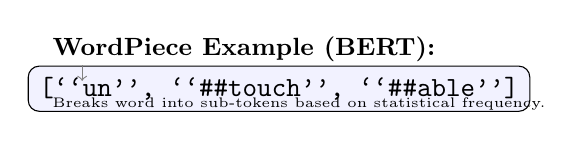
\begin{tikzpicture}
    % WordPiece example
    \node[anchor=west] at (0, 0.5) {\small \textbf{WordPiece Example (BERT):}};
    \node[draw, fill=blue!5, rounded corners, inner sep=4pt] at (3, 0) {\texttt{[``un'', ``\#\#touch'', ``\#\#able'']}};
    \draw[->, gray, thin] (0.5, 0.3) -- (0.5, 0.1);
    \node[anchor=west] at (0, -0.2) {\tiny Breaks word into sub-tokens based on statistical frequency.};
\end{tikzpicture}

\end{center}
\end{frame}

\begin{frame}[shrink=10]{Index Compression: Why It Matters}
\begin{block}{The Bottleneck}
Modern CPUs: 3+ GHz, billions of operations/second \\
Modern SSDs: 500 MB/s read speed

\vspace{0.5em}

\textbf{Decompression:} 2-5 GB/s \\
\textbf{Reading uncompressed:} 0.5 GB/s

\vspace{0.5em}

$\rightarrow$ \textbf{Reading compressed data is faster!}
\end{block}

\vspace{1em}

\begin{exampleblock}{Real Impact}
\textbf{Collection:} 10M documents, 100 words each \\
\textbf{Uncompressed index:} 10 GB \\
\textbf{Compressed (5$\times$):} 2 GB

\vspace{0.5em}

Benefits:
\begin{itemize}
    \item More index fits in RAM (faster queries)
    \item Lower storage costs
    \item Faster I/O (disk $\rightarrow$ memory)
\end{itemize}
\end{exampleblock}
\end{frame}

\begin{frame}[shrink=10]{Gap Encoding: The Key Insight}
\textbf{Original posting list (docIDs):}
\begin{center}
[5, 127, 214, 215, 512, 1024, 2048, 10239]
\end{center}

\vspace{0.5em}

\textbf{Observation:} Most gaps between consecutive docIDs are small

\vspace{0.5em}

\textbf{Store gaps instead:}
\begin{center}
[5, 122, 87, 1, 297, 512, 1024, 8191]
\end{center}

\vspace{1em}

\begin{block}{Why This Helps}
\textbf{Original:} Numbers range 5-10,239 $\rightarrow$ need 14 bits each \\
\textbf{Gaps:} Most numbers small ($<$ 256) $\rightarrow$ need fewer bits

\vspace{0.5em}

Small numbers compress much better!
\end{block}

\vspace{1em}

\begin{alertblock}{Decoding}
Sequential only: $\text{docID}_i = \text{docID}_{i-1} + \text{gap}_i$
\end{alertblock}
\end{frame}

\begin{frame}[shrink=10]{Variable Byte (VB) Encoding}
\begin{block}{Core Idea}
Use 1 byte for small numbers, multiple bytes for large numbers
\begin{itemize}
    \item 7 bits for data
    \item 1 bit (MSB) for continuation: 1 = last byte, 0 = more bytes follow
\end{itemize}
\end{block}

\vspace{1em}

\begin{table}
\centering
\begin{tabular}{lll}
\toprule
\textbf{Number} & \textbf{Binary} & \textbf{VB Encoding} \\
\midrule
5 & 101 & \texttt{1\_0000101} (1 byte) \\
122 & 1111010 & \texttt{1\_1111010} (1 byte) \\
824 & 1100111000 & \texttt{0\_0000110 1\_0111000} (2 bytes) \\
\bottomrule
\end{tabular}
\end{table}

\vspace{1em}

\textbf{Example compression:}
\begin{itemize}
    \item Gaps: [5, 122, 87, 1] $\rightarrow$ 4 bytes (VB encoded)
    \item Uncompressed: 16 bytes (4 $\times$ 32-bit integers)
    \item \textbf{Compression ratio: 4$\times$}
\end{itemize}
\end{frame}

\begin{frame}[shrink=5]{VB Encoding: Step-by-Step Example}
\textbf{Encode 824:}

\vspace{0.5em}

\begin{enumerate}
    \item Binary representation: 1100111000 (10 bits needed)
    \item Needs 2 bytes (10 $>$ 7)
    \item Split into 7-bit chunks from right: \\
    \begin{itemize}
        \item Lower 7 bits: 0111000
        \item Upper bits: 0000110
    \end{itemize}
    \item First byte (higher bits): \texttt{0\_0000110} (continuation = 0)
    \item Second byte (lower bits): \texttt{1\_0111000} (continuation = 1, last byte)
    \item Result: \texttt{00000110 10111000}
\end{enumerate}

\vspace{1em}

\textbf{Decode:}
\begin{enumerate}
    \item Read bytes until continuation bit = 1
    \item Strip continuation bits: \texttt{0000110 0111000}
    \item Concatenate: 0000110\_0111000 = 1100111000 = 824 \faCheck 
\end{enumerate}
\end{frame}

\begin{frame}[shrink=5]{Compression in Practice}
\begin{block}{Typical Results}
\begin{itemize}
    \item VB encoding: 3-4$\times$ compression
    \item More sophisticated methods (PForDelta): 6-10$\times$ compression
    \item Dictionary compression (front coding): 30-50% savings
\end{itemize}
\end{block}

\vspace{1em}

\begin{exampleblock}{Production Systems}
\begin{itemize}
    \item \textbf{Lucene/Elasticsearch:} Uses FOR (Frame of Reference) with SIMD
    \item \textbf{Google:} Custom compression optimized for their hardware
    \item \textbf{Your projects:} VB encoding is good enough (simple, effective)
\end{itemize}
\end{exampleblock}

\vspace{1em}

\begin{alertblock}{Key Takeaway}
Compression is not optional --- it makes systems \textbf{faster} and cheaper
\end{alertblock}
\end{frame}

\begin{frame}[fragile,shrink=5]{PyTerrier Demo: Sparse Indexing}
\begin{lstlisting}[language=Python, basicstyle=\ttfamily\tiny]
import pyterrier as pt
pt.init()

# Load dataset
dataset = pt.get_dataset('irds:vaswani')

# Index documents (builds inverted index with compression)
indexer = pt.IterDictIndexer("./vaswani_index", overwrite=True)
index_ref = indexer.index(dataset.get_corpus_iter())
print("Indexing complete!")

# Build retriever (uses BM25 scoring)
bm25 = pt.BatchRetrieve(index_ref, wmodel="BM25")

# Search
results = bm25.search("aerodynamic flow over wings")
print(results[['docno', 'score', 'rank']].head())

# Evaluate on full test set
evaluation = pt.Experiment(
    [bm25],
    dataset.get_topics(),
    dataset.get_qrels(),
    eval_metrics=["map", "ndcg_cut_10", "P_10"]
)
print(evaluation)
#    name       map  ndcg_cut_10      P_10
# 0  BM25  0.234567     0.456789  0.345678
\end{lstlisting}

\textbf{This is production-ready sparse retrieval!}
\end{frame}

% ====================================================================
% SECTION 2: DENSE INDEXING (NEURAL)
% ====================================================================
\section{Dense Vector Indexing for Neural Retrieval}

\begin{frame}[shrink=10]{The Shift to Dense Vectors}
\begin{columns}
\begin{column}{0.48\textwidth}
\begin{block}{Sparse (BM25)}
\textbf{Doc:} ``car problems''

\vspace{0.5em}

\textbf{Representation:}
\begin{itemize}
    \item Dimensions: 30,000 (vocab)
    \item car: 1
    \item problems: 1
    \item All else: 0
    \item \textbf{99.99\% zeros}
\end{itemize}

\vspace{0.5em}

\textbf{Limitation:} \\
Misses ``automobile issues''
\end{block}
\end{column}

\begin{column}{0.48\textwidth}
\begin{block}{Dense (Neural)}
\textbf{Doc:} ``car problems''

\vspace{0.5em}

\textbf{Representation:}
\begin{itemize}
    \item Dimensions: 768
    \item {[0.23, -0.41, 0.87, \dots]}
    \item All non-zero
    \item \textbf{100\% dense}
\end{itemize}

\vspace{0.5em}

\textbf{Advantage:} \\
Matches ``automobile issues'' \\
(similar embedding!)
\end{block}
\end{column}
\end{columns}

\vspace{1em}

\begin{alertblock}{The Problem}
Can't use inverted index (no discrete terms) \\
Need: \textbf{Approximate Nearest Neighbor (ANN) search}
\end{alertblock}
\end{frame}

\begin{frame}[shrink=15]{The ANN Search Problem}
\begin{block}{Task}
\textbf{Given:}
\begin{itemize}
    \item Collection of $N$ vectors: $\{\vec{d}_1, \vec{d}_2, \ldots, \vec{d}_N\}$
    \item Query vector: $\vec{q}$
\end{itemize}

\textbf{Find:} $k$ vectors most similar to $\vec{q}$ (typically cosine similarity)
\end{block}

\vspace{1em}

\begin{alertblock}{Naive Solution: Exact Search}
Compare query to \textbf{all} $N$ vectors: $O(N \cdot d)$

\vspace{0.5em}

For $N = 10^9$ docs, $d = 768$ dimensions: \\
768 billion operations $\rightarrow$ \textbf{too slow!} ($>$1 second even on GPU)
\end{alertblock}

\vspace{1em}

\begin{exampleblock}{Solution: Approximate Nearest Neighbor (ANN)}
Trade exactness for speed: find \textit{approximately} top-$k$ \\
Typical accuracy: 90-99\% recall (good enough for IR!)
\end{exampleblock}
\end{frame}

\begin{frame}[shrink=5]{ANN: Accuracy-Speed Trade-off}
\begin{center}
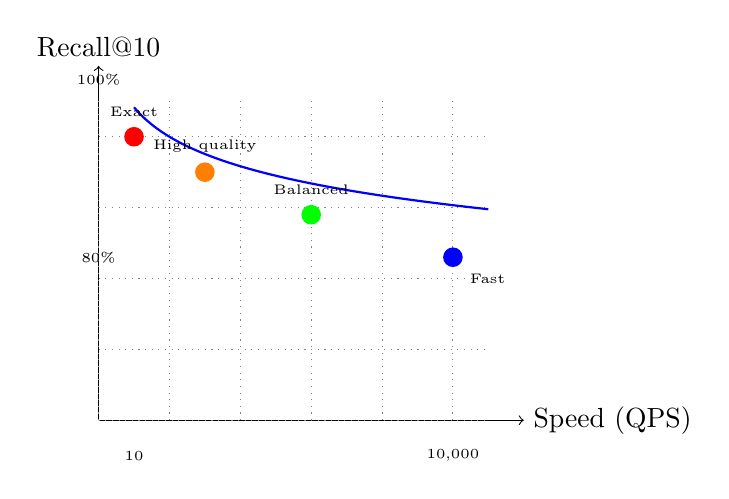
\begin{tikzpicture}[scale=0.9]
    % Axes
    \draw[->] (0,0) -- (6,0) node[right] {Speed (QPS)};
    \draw[->] (0,0) -- (0,5) node[above] {Recall@10};
    
    % Grid
    \draw[gray, dotted] (0,0) grid (5.5,4.5);
    
    % Curve
    \draw[blue, thick, domain=0.5:5.5, samples=100] 
        plot (\x, {4 - 0.6*ln(\x)});
    
    % Points
    \node[circle, fill=red, inner sep=2.5pt, label=above:{\tiny Exact}] at (0.5, 4) {};
    \node[circle, fill=orange, inner sep=2.5pt, label=above:{\tiny High quality}] at (1.5, 3.5) {};
    \node[circle, fill=green, inner sep=2.5pt, label=above:{\tiny Balanced}] at (3, 2.9) {};
    \node[circle, fill=blue, inner sep=2.5pt, label=below right:{\tiny Fast}] at (5, 2.3) {};
    
    % Labels
    \node at (0, 4.8) {\tiny 100\%};
    \node at (0, 2.3) {\tiny 80\%};
    \node at (0.5, -0.5) {\tiny 10};
    \node at (5, -0.5) {\tiny 10,000};
\end{tikzpicture}

\end{center}

\vspace{0.5em}

\textbf{Typical operating points:}
\begin{itemize}
    \item \textbf{High quality:} 95-99\% recall @ 100-500 QPS (production RAG)
    \item \textbf{Balanced:} 90-95\% recall @ 500-2000 QPS (most use cases)
    \item \textbf{Fast:} 80-90\% recall @ 2000-10,000 QPS (first-stage retrieval)
\end{itemize}
\end{frame}

\begin{frame}{From Text to Index: A Unified View}
\begin{center}
\begin{tikzpicture}[scale=0.5, every node/.style={scale=0.5}]
    % Raw Input
    \IRBox{text}{(0,0)}{Raw Text}{Collection}{primary}
    
    % Sparse branch
    \IRBox{tokens}{(4,1.5)}{Tokenization}{Lexical Phase}{primary}
    \IRBox{ids}{(8,1.5)}{Term IDs}{Mapping}{primary}
    \IRBox{sindex}{(12,1.5)}{Inverted Index}{Static Index}{secondary}
    
    % Dense branch
    \IRBox{mtoken}{(4,-1.5)}{Model Tokenizer}{Neural Phase}{accent}
    \IRBox{embed}{(8,-1.5)}{Encoding (BERT)}{Vectorization}{accent}
    \IRBox{dindex}{(12,-1.5)}{ANN Index}{Dynamic Index}{secondary}
    
    % Target
    \IRBox{res}{(16,0)}{Ranked Candidates}{Top-$k$ List}{emph}
    
    % Sparse Connections
    \IRArrow{text.north}{tokens.west}{Sparse Pipeline}
    \IRArrow{tokens}{ids}{}
    \IRArrow{ids}{sindex}{}
    \IRArrow{sindex}{res.north}{}
    
    % Dense Connections
    \IRArrow{text.south}{mtoken.west}{Dense Pipeline}
    \IRArrow{mtoken}{embed}{}
    \IRArrow{embed}{dindex}{}
    \IRArrow{dindex}{res.south}{}
\end{tikzpicture}

\end{center}

\vspace{1em}
\begin{exampleblock}{Key Distinction}
\textbf{Sparse:} Matches exact characters (lexical). \\
\textbf{Dense:} Matches numerical meaning (semantic).
\end{exampleblock}
\end{frame}

\begin{frame}[shrink=5]{The Standard ANN Approach: IVF + PQ}
\begin{enumerate}
    \item \textbf{Clustering-Based (IVF)}
    \begin{itemize}
        \item Cluster vectors with k-means
        \item Search only in nearest clusters
        \item \textcolor{green}{\faCheck } Fast, scalable
        \item \textcolor{red}{\faTimes } Lower accuracy without tuning
    \end{itemize}
    
    \item \textbf{Product Quantization (PQ)}
    \begin{itemize}
        \item Compress vectors aggressively (32$\times$)
        \item Approximate distances in compressed space
        \item \textcolor{green}{\faCheck } Very memory-efficient
        \item \textcolor{red}{\faTimes } Moderate accuracy loss
    \end{itemize}
    
    \item \textbf{Combined (IVF + PQ)}
    \begin{itemize}
        \item Use clustering to narrow search area
        \item Use compression to fit index in RAM and speed up distance calculation
        \item \textcolor{green}{\faCheck } \textbf{The industry standard for large-scale RAG}
    \end{itemize}
\end{enumerate}
\end{frame}

% HNSW section removed for focus on IVF+PQ

\begin{frame}[shrink=10]{IVF: Inverted File Index (for Vectors!)}
\begin{block}{Core Idea}
Cluster vectors, then search only in nearest clusters
\end{block}

\vspace{0.5em}

\begin{center}
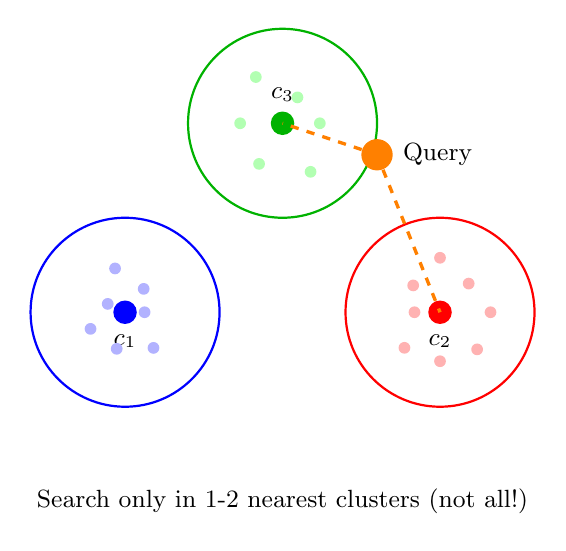
\begin{tikzpicture}[scale=0.8]
    % Cluster 1
    \draw[thick, blue] (0,0) circle (1.5);
    \node[circle, fill=blue, inner sep=3pt, label=below:{\small $c_1$}] at (0,0) {};
    \foreach \i in {1,...,7} {
        \pgfmathsetmacro{\angle}{360/7*\i}
        \pgfmathsetmacro{\r}{0.3+0.5*rnd}
        \node[circle, fill=blue!30, inner sep=1.5pt] at (\angle:\r) {};
    }
    
    % Cluster 2
    \draw[thick, red] (5,0) circle (1.5);
    \node[circle, fill=red, inner sep=3pt, label=below:{\small $c_2$}] at (5,0) {};
    \foreach \i in {1,...,8} {
        \pgfmathsetmacro{\angle}{360/8*\i}
        \pgfmathsetmacro{\r}{0.3+0.6*rnd}
        \node[circle, fill=red!30, inner sep=1.5pt] at ($(5,0)+(\angle:\r)$) {};
    }
    
    % Cluster 3
    \draw[thick, green!70!black] (2.5,3) circle (1.5);
    \node[circle, fill=green!70!black, inner sep=3pt, label=above:{\small $c_3$}] at (2.5,3) {};
    \foreach \i in {1,...,6} {
        \pgfmathsetmacro{\angle}{360/6*\i}
        \pgfmathsetmacro{\r}{0.4+0.5*rnd}
        \node[circle, fill=green!30, inner sep=1.5pt] at ($(2.5,3)+(\angle:\r)$) {};
    }
    
    % Query
    \node[circle, fill=orange, inner sep=4pt, label=right:{\small Query}] (q) at (4,2.5) {};
    
    % Distance to nearest clusters
    \draw[dashed, orange, very thick] (q) -- (2.5,3);
    \draw[dashed, orange, very thick] (q) -- (5,0);
    
    \node at (2.5,-3.0) {\small Search only in 1-2 nearest clusters (not all!)};
\end{tikzpicture}

\end{center}
\end{frame}

\begin{frame}[shrink=20]{IVF: Construction and Search}
\begin{block}{Construction}
\begin{algorithmic}[1]
\STATE Run k-means on all vectors $\rightarrow$ get $k$ cluster centers (e.g., $k=1000$)
\STATE Assign each vector to its nearest cluster center
\STATE Build inverted lists: cluster $i$ $\rightarrow$ [vector IDs in cluster $i$]
\end{algorithmic}
\end{block}

\vspace{1em}

\begin{block}{Search}
\begin{algorithmic}[1]
\STATE \textbf{Input:} Query $\vec{q}$, $n_{\text{probe}}$ (clusters to search), $k$
\STATE Compute distance from $\vec{q}$ to all cluster centers
\STATE Select $n_{\text{probe}}$ nearest cluster centers
\STATE $\text{candidates} \gets []$
\FOR{each selected cluster}
    \STATE Fetch all vectors in cluster
    \STATE Compute exact distances to $\vec{q}$
    \STATE Add to candidates
\ENDFOR
\STATE Sort candidates by distance, return top-$k$
\end{algorithmic}
\end{block}

\vspace{0.5em}

\textbf{Key parameter:} $n_{\text{probe}}$ (1 = fast/low recall, 100 = slow/high recall)
\end{frame}

\begin{frame}[shrink=10]{Product Quantization: Compression}
\begin{block}{Goal}
Compress 768-dim vector (3072 bytes) to 96 bytes (32$\times$ compression!)
\end{block}

\vspace{1em}

\textbf{Method:}
\begin{enumerate}
    \item \textbf{Split} each vector into $m$ subvectors (e.g., $m=96$ subvectors of 8 dims)
    \item \textbf{Quantize} each subvector: assign to nearest centroid (256 centroids)
    \item \textbf{Store} centroid ID (1 byte) instead of full subvector
\end{enumerate}

\vspace{1em}

\begin{exampleblock}{Example}
\textbf{Original:} [0.23, -0.41, 0.87, 0.12, -0.34, 0.56, 0.78, -0.23, ...] (768 floats)

\textbf{Split into 96 subvectors:}
\begin{itemize}
    \item Subvec 1: [0.23, -0.41, 0.87, 0.12, -0.34, 0.56, 0.78, -0.23] $\rightarrow$ Centroid 42
    \item Subvec 2: [0.45, 0.67, -0.12, 0.89, 0.34, -0.56, 0.23, 0.11] $\rightarrow$ Centroid 123
    \item ... (96 total)
\end{itemize}

\textbf{Compressed:} [42, 123, 7, 89, ...] (96 bytes)
\end{exampleblock}
\end{frame}

\begin{frame}[shrink=10]{Product Quantization: Distance Approximation}
\begin{block}{Key Insight}
Can approximate distances using only centroid IDs (no need to decompress!)
\end{block}

\vspace{1em}

\textbf{Algorithm:}
\begin{enumerate}
    \item \textbf{Precompute} distance table: query subvector to all centroids
    \begin{itemize}
        \item For each of 96 subspaces
        \item For each of 256 centroids
        \item Total: 96 $\times$ 256 = 24,576 distances (computed once per query)
    \end{itemize}
    
    \item \textbf{For each document:}
    \begin{itemize}
        \item Approximate distance = $\sum_{i=1}^{96} \text{distTable}_i[\text{code}_i]$
        \item Just 96 lookups + additions (very fast!)
    \end{itemize}
\end{enumerate}

\vspace{1em}

\begin{exampleblock}{Performance}
\begin{itemize}
    \item \textbf{Memory:} 32$\times$ compression (3GB $\rightarrow$ 96MB for 1M vectors)
    \item \textbf{Speed:} 10-100$\times$ faster than exact distance
    \item \textbf{Accuracy:} 80-95\% recall typical
\end{itemize}
\end{exampleblock}
\end{frame}

\begin{frame}[shrink=10]{IVF + PQ: The Production Standard}
\begin{block}{Best of Both Worlds}
Combine IVF (clustering) with PQ (compression)
\end{block}

\vspace{1em}

\textbf{Architecture:}
\begin{enumerate}
    \item \textbf{Offline:} Cluster vectors into $k$ clusters (IVF)
    \item \textbf{Offline:} Compress vectors with PQ
    \item \textbf{Online:} Find $n_{\text{probe}}$ nearest clusters
    \item \textbf{Online:} Search within those clusters using PQ distances
\end{enumerate}

\vspace{1em}

\begin{exampleblock}{Real-World Impact}
\textbf{Facebook/Meta AI Similarity Search (FAISS):}
\begin{itemize}
    \item 1 billion vectors $\times$ 768 dims $\times$ 4 bytes = \textbf{3 TB}
    \item With IVFPQ: 1 billion vectors $\times$ 64 bytes = \textbf{64 GB}
    \item \textbf{50$\times$ memory reduction!}
    \item Still achieves 90-95\% recall with proper tuning
\end{itemize}
\end{exampleblock}

\vspace{0.5em}

\textbf{Used by:} Meta, OpenAI, many large-scale systems
\end{frame}

\begin{frame}[fragile,shrink=20]{FAISS Demo: Dense Indexing (IVF+PQ)}
\begin{lstlisting}[language=Python, basicstyle=\ttfamily\tiny]
import numpy as np
import faiss

# Simulate document embeddings (100k docs, 768 dims)
dimension = 768
n_docs = 100000
doc_embeddings = np.random.randn(n_docs, dimension).astype('float32')
faiss.normalize_L2(doc_embeddings)  # For cosine similarity

# === 1. Training & Building IVF+PQ index ===
n_clusters = 100  # Number of clusters (centroids)
m_subvectors = 96 # Number of PQ subvectors (768/96 = 8 dims each)
bits = 8          # Bits per subvector (256 centroids per subspace)

quantizer = faiss.IndexFlatL2(dimension)
index = faiss.IndexIVFPQ(quantizer, dimension, n_clusters, m_subvectors, bits)

print("Training index...")
index.train(doc_embeddings) # PQ needs training to find centroids
index.add(doc_embeddings)
print(f"Total docs indexed: {index.ntotal}")

# === 2. Search ===
query = np.random.randn(1, dimension).astype('float32')
faiss.normalize_L2(query)

index.nprobe = 10  # Search 10 nearest clusters
distances, indices = index.search(query, k=10)

print("Top 10 document indices:", indices[0])
print("Approximate distances:", distances[0])

# Memory usage (approximation)
# Uncompressed: 100,000 * 768 * 4 bytes = 307.2 MB
# IVFPQ: 100,000 * 96 bytes = 9.6 MB (~32x smaller!)
\end{lstlisting}
\end{frame}

% Remnants of old ranking/hybrid code removed

% ====================================================================
% SECTION 4: DESIGN DECISIONS
% ====================================================================
\section{Design Decisions: When to Use What}

\begin{frame}{The Decision Matrix: Scale vs. Precision}
\begin{table}
\centering
\small
\begin{tabular}{lcc}
\toprule
\textbf{Aspect} & \textbf{Sparse (Inverted Index)} & \textbf{Dense (IVF+PQ)} \\
\midrule
Best for & Exact Match, Rare Keywords & Semantic Similarity \\
Recall & Medium (High for entities) & High (Semantic) \\
Precision & Very High & High \\
Latency & 5-20ms & 10-50ms \\
Memory & Low & Low-Medium (due to compression) \\
Scalability & Excellent & Excellent (with IVF) \\
Explainability & High & Low (Black box) \\
\bottomrule
\end{tabular}
\end{table}

\vspace{1em}

\begin{block}{Production Wisdom}
\begin{itemize}
    \item Use \textbf{Sparse} when you need to find exact names, model numbers, or unique terms.
    \item Use \textbf{Dense} when users ask questions in natural language or use synonyms.
\end{itemize}
\end{block}
\end{frame}

% Removed use cases focusing on Hybrid Search

\begin{frame}[shrink=10]{Case Study: Academic Paper Search (100M+)}
\begin{exampleblock}{Scenario}
Research search engine with 100M papers (arXiv, PubMed, etc.)
\end{exampleblock}

\textbf{The Challenge:}
\begin{itemize}
    \item Cannot hold 100M raw vectors in RAM (300GB+).
    \item Users need both exact titles (Sparse) and broad conceptual search (Dense).
\end{itemize}

\begin{block}{The Strategy: IVF+PQ}
\begin{itemize}
    \item \textbf{Sparse (BM25):} Index title, authors, abstracts for keyword matching.
    \item \textbf{Dense (IVF+PQ):} 
        \begin{itemize}
            \item Cluster into 10k centroids (high speed).
            \item Compress vectors 32$\times$ (fits on a single server!).
        \end{itemize}
\end{itemize}
\end{block}

\textbf{Result:} Billion-scale search with low latency and low cost.
\end{frame}

% Removed HNSW/Hybrid trade-off slides

\begin{frame}[shrink=5]{Common Pitfalls and Solutions}
\begin{alertblock}{Pitfall 1: Using Only Dense for Entity-Heavy Domains}
\textbf{Problem:} Query ``Python 3.11 release date'' $\rightarrow$ matches ``snake release from zoo''

\textbf{Solution:} Use hybrid! BM25 catches ``Python 3.11'' exactly
\end{alertblock}

\begin{alertblock}{Pitfall 2: Not Tuning ANN Parameters}
\textbf{Problem:} Using default \texttt{ef\_search=16} $\rightarrow$ only 80\% recall

\textbf{Solution:} Tune on dev set. Start \texttt{ef\_search=64}, increase until recall plateaus
\end{alertblock}

\begin{alertblock}{Pitfall 3: Inconsistent Preprocessing}
\textbf{Problem:} Index with stemming, query without $\rightarrow$ no matches!

\textbf{Solution:} Same preprocessing for both. For embeddings: no stemming!
\end{alertblock}

\begin{alertblock}{Pitfall 4: Forgetting to Normalize Vectors}
\textbf{Problem:} Using unnormalized embeddings $\rightarrow$ Euclidean distance $\neq$ cosine similarity

\textbf{Solution:} Always normalize: \texttt{faiss.normalize\_L2(embeddings)}
\end{alertblock}
\end{frame}

\begin{frame}[shrink=20]{Production Checklist}
\textbf{Before deploying, verify:}

\vspace{0.5em}

\begin{columns}
\begin{column}{0.48\textwidth}
\textbf{Sparse Index:}
\begin{itemize}
    \item[$\square$] Compression enabled
    \item[$\square$] Stop words handled
    \item[$\square$] Stemming appropriate
    \item[$\square$] Field boosting configured
    \item[$\square$] Metadata filterable
\end{itemize}

\vspace{0.5em}

\textbf{Dense Index (IVF+PQ):}
\begin{itemize}
    \item[$\square$] Vectors normalized
    \item[$\square$] Number of probes ($n\_probe$) tuned
    \item[$\square$] Memory budget met
    \item[$\square$] PQ training data is representative
\end{itemize}
\end{column}

\begin{column}{0.48\textwidth}
\textbf{Monitoring:}
\begin{itemize}
    \item[$\square$] Track recall@k (vs. exact search)
    \item[$\square$] Monitor p95/p99 latency
    \item[$\square$] Alert on index growth
    \item[$\square$] Log query/document drift
\end{itemize}
\end{column}
\end{columns}
\end{frame}

\begin{frame}[shrink=20]{Modern IR Infrastructure Examples}
\begin{block}{Production RAG (Cloud/Managed)}
\begin{itemize}
    \item \textbf{Embedding:} OpenAI \texttt{text-embedding-3-small}
    \item \textbf{Vector DB:} Pinecone, Qdrant, or Milvus Managed.
    \item \textbf{Candidate Generation:} Dense-first (IVF or HNSW hidden by provider).
    \item \textbf{LLM:} GPT-4o / Claude 3.5 Sonnet.
\end{itemize}
\end{block}

\begin{block}{Large Scale Open Source}
\begin{itemize}
    \item \textbf{Sparse:} Elasticsearch / OpenSearch (self-hosted).
    \item \textbf{Dense:} FAISS (IVF+PQ) for billionaire-scale efficiency.
    \item \textbf{Language:} Python / C++ for performance.
    \item \textbf{Next Step:} Re-ranking with Cross-encoders (Lecture 4).
\end{itemize}
\end{block}
\end{frame}



% ====================================================================
% WRAP-UP
% ====================================================================
\section{Summary and Next Steps}

\begin{frame}[shrink=5]{What We Covered Today}
\begin{enumerate}
    \item \textbf{Sparse Indexing (Classical)}
    \begin{itemize}
        \item Inverted index structure
        \item Text preprocessing pipeline
        \item Compression (Gap encoding + VB)
        \item PyTerrier demo
    \end{itemize}
    
    \item \textbf{Dense Indexing (Neural)}
    \begin{itemize}
        \item Why ANN search is needed
        \item IVF+PQ: The standard for scale (Clustering + Compression)
        \item FAISS demo
    \end{itemize}
    
    \item \textbf{Design Decisions}
    \begin{itemize}
        \item Modern IR Pipeline (Candidate Generation)
        \item Traditional IR vs. RAG
        \item Scaling to billions of documents
    \end{itemize}
\end{enumerate}
\end{frame}

\begin{frame}[shrink=5]{Key Takeaways}
\begin{block}{1. Inverted Indexes are the Backbone}
Keyword matching is essential for exact queries and entities. Don't throw away BM25!
\end{block}

\begin{block}{2. Dense Retrieval Enables Semantic Search}
Embeddings capture meaning, but require ANN techniques like IVF+PQ to work at scale.
\end{block}

\begin{block}{3. Candidate Generation is the Bottleneck}
Fast indexing determines how many documents your re-rankers or LLMs can "see".
\end{block}

\begin{block}{4. Scalability requires Compression}
Techniques like Product Quantization (PQ) are vital for fitting large indexes in RAM.
\end{block}
\end{frame}

\begin{frame}[shrink=10]{Connection to Next Lectures}
\textbf{Lecture 3: Ranking Models}
\begin{itemize}
    \item BM25 scoring uses inverted indexes we built today
    \item Query expansion (RM3) operates on sparse retrieval
    \item Language models for better ranking
\end{itemize}

\vspace{0.5em}

\textbf{Lecture 4: Transformer Re-rankers}
\begin{itemize}
    \item Re-rank candidates from hybrid retrieval
    \item Cross-encoders (BERT) for precision
    \item Two-stage: retrieve (today) $\rightarrow$ re-rank (lecture 4)
\end{itemize}

\vspace{0.5em}

\textbf{Lecture 5: Dense Retrieval (Deep Dive)}
\begin{itemize}
    \item Bi-encoders in detail
    \item Training dense retrievers
    \item We already know ANN indexing!
\end{itemize}

\vspace{0.5em}

\textbf{Lecture 6: Learning to Rank}
\begin{itemize}
    \item Combine sparse + dense scores optimally
    \item Learn fusion weights from data
    \item Put it all together
\end{itemize}
\end{frame}

\begin{frame}[shrink=10]{Assignment 2: From Sparse to Dense Retrieval}
\textbf{Due:} 2 weeks

\vspace{1em}

\textbf{Tasks:}
\begin{enumerate}
    \item \textbf{Sparse Indexing (40 pts)}
    \begin{itemize}
        \item Build inverted index with PyTerrier.
        \item Measure effect of compression (VB) on index size.
    \end{itemize}
    
    \item \textbf{Dense Indexing (40 pts)}
    \begin{itemize}
        \item Build IVF+PQ index with FAISS on 100k vectors.
        \item Measure recall vs. exact search as you change \texttt{n\_probe}.
    \end{itemize}
    
    \item \textbf{Analysis (20 pts)}
    \begin{itemize}
        \item Compare latency and memory usage of Sparse vs. Dense.
        \item Identify query types where each method fails.
    \end{itemize}
\end{enumerate}
\end{frame}

\begin{frame}[shrink=10]{Resources}
\begin{block}{Documentation}
\begin{itemize}
    \item PyTerrier: \url{https://pyterrier.readthedocs.io}
    \item FAISS: \url{https://github.com/facebookresearch/faiss/wiki}
    \item Sentence Transformers: \url{https://www.sbert.net}
\end{itemize}
\end{block}

\begin{block}{Papers (Optional Reading)}
\begin{itemize}
    \item HNSW: Malkov \& Yashunin (2018) - "Efficient and robust approximate nearest neighbor search using Hierarchical Navigable Small World graphs"
    \item Product Quantization: Jégou et al. (2011) - "Product quantization for nearest neighbor search"
    \item Hybrid Search: Lin et al. (2021) - "A Few Brief Notes on DeepImpact, COIL, and a Conceptual Framework for Information Retrieval Techniques"
\end{itemize}
\end{block}

\begin{block}{Tools}
\begin{itemize}
    \item Vector databases: Pinecone, Weaviate, Qdrant, Milvus
    \item Elasticsearch 8.0+ (native kNN + BM25)
    \item Vespa (Yahoo's search engine, open source)
\end{itemize}
\end{block}
\end{frame}

\begin{frame}[shrink=10]{Questions?}
\begin{center}
\Huge Questions?

\vspace{2em}

\Large
Office Hours: [Your time]

\vspace{1em}

Email: [Your email]

\vspace{2em}

\normalsize
\textbf{Next Class: Lecture 3 --- Ranking Models}

\vspace{0.5em}

We'll use the indexes we built today to implement BM25, \\
language models, and query expansion!

\vspace{1em}

\textbf{Start the assignment early} --- building a hybrid system takes time!
\end{center}
\end{frame}

\end{document}